% Required TeX compilation engine: XeLaTeX
\documentclass[a4paper,14pt]{extarticle}

% Поля
\usepackage[left=3cm,right=1.5cm,top=2cm,bottom=2cm]{geometry}

% Кириллица с поддержкой переносов
\usepackage[russian]{babel}
\usepackage[autostyle=true]{csquotes}
\usepackage{microtype}
\tolerance=1000
\sloppy

% Таблицы
\usepackage{array}
\usepackage{booktabs}

% Код
\usepackage{listings}
\usepackage{xcolor}
\lstset{
    basicstyle=\ttfamily\small,
    keywordstyle=\color{blue},
    commentstyle=\color{gray},
    numbers=left,
    numberstyle=\tiny\color{gray},
    frame=single,
    breaklines=true,
    tabsize=4
}

% Графика
\usepackage{graphicx}
\usepackage{amssymb}

% Шрифты
\usepackage{fontspec}
\setmainfont{Times New Roman}

% Интервал
\usepackage{setspace}
\onehalfspacing

% Красная строка
\usepackage{indentfirst}
\setlength{\parindent}{1.25cm}

% Цвет текста
\usepackage{xcolor}
\color{black}

% Создание оглавления
\usepackage{hyperref}
\newcommand{\nosubsection}[1]{%
  \refstepcounter{subsection}%
  \subsection*{\thesubsection\hspace{1em}#1}%
}

% Оглавление на отдельной странице
\usepackage{tocloft}
\renewcommand{\cftsecleader}{\cftdotfill{\cftdotsep}}

% Оформление источников по ГОСТу
\usepackage[style=gost-numeric,sortlocale=ru_RU,natbib=true]{biblatex}
\addbibresource{bibliography.bib}

\begin{document}

\begin{titlepage}
  \begin{center}
    МИНИСТЕРСТВО НАУКИ И ВЫСШЕГО ОБРАЗОВАНИЯ РОССИЙСКОЙ ФЕДЕРАЦИИ\\
    Федеральное государственное автономное образовательное учреждение высшего образования\\
    \textbf{«Национальный исследовательский Нижегородский государственный университет им. Н.И. Лобачевского» (ННГУ)}\\
    \vspace*{\fill}
    {\LARGE Разработка компилятора.\\и тд}\\
    \vspace{2cm}
  \end{center}
  \hfill
  \begin{minipage}{0.4\textwidth}
    \raggedright
    \textbf{Выполнил:}\\
    Власов Максим Сергеевич,\\
    студент группы 3823М1ПМкн\\
  \end{minipage}
  \vspace*{\fill}
  \begin{center}
    Нижний Новгород\\
    2025
  \end{center}
\end{titlepage}

\newpage
\setcounter{page}{2}
\tableofcontents

\newpage
\section*{Введение}
\addcontentsline{toc}{section}{Введение}

В 1957 году появился первый в мире компилятор языка Фортран, который был создан Д. Бэкусом. Компилятор позволял генерировать достаточно быстрый объектный код. До этого времени процесс создания компиляторов не был формализован, и отсутствовало понимание, что является основой компиляторов.

С развитием формальной теории языков и математической лингвистики стали появляться новые все более сложные языки программирования. Также развивались понятия генерации объектного кода, машинно-зависимых инструкций. Хотя компьютеры и их составляющие из года в год становятся лучше и лучше, основы построения компиляторов остаются неизменными.

Итак, настоящая работа будет посвящена разработке компилятора.

\newpage
\section*{Постановка задачи}
\addcontentsline{toc}{section}{Постановка задачи}

Требуется разработать и реализовать упрощенный компилятор Python-подобного статически типизированного языка с поддержкой основных языковых конструкций.  Для достижения цели проекта были поставлены следующие задачи:

\begin{itemize}
    \item определить подмножество реализуемого синтаксиса языка Python;
    \item изучить литературу о структуре и способах разработки существующих компиляторов, а также моделях исполнения программ;
    \item разработать архитектуру модулей компилятора и организацию взаимодействия между ними для выбранного языка;
    \item реализовать описанные модули, произвести их тестирование.
\end{itemize}

Разработка проекта велась коллективом в составе Власова М. С., Тактаева А. А., Шагова М. А., студентов группы 381806-1. Разделы 1, 2, 3, 6 настоящей работы отражают результаты, полученные совместно с равным вкладом всех участников коллектива. Разделы 4, 5 отражают личный вклад автора в проект.

В рамках работы были подробно описаны и реализованы следующие модули:

\begin{itemize}
    \item синтаксический анализатор;
    \item генератор промежуточного представления LLVM IR;
\end{itemize}

а также сопутствующие структуры данных.

\newpage
\section{Обзор предметной области}
\label{sec:subject_overview}

Компилятор -- программа, способная получать на вход код программы, написанной на одном (исходном) языке и транслировать его в код эквивалентной программы на другом (целевом) языке.
Важной ролью компилятора является обнаружение ошибок во время трансляции кода исходной программы и сообщение о них пользователю.
Если целевая программа является машиночитаемой (исполняемой компьютером), она может быть вызвана пользователем для обработки входных и получения выходных данных.
Этот подход используется в таких языках программирования, как Си, C++, Go и т. д.

Интерпретатор -- это другой распространённый вид программ для обработки языков.
Вместо создания целевой программы в процессе трансляции интерпретатор непосредственно выполняет операции, указанные в коде исходной программы, с использованием предоставленных пользователем входных данных.
Интерпретируемыми языками являются, например, Python, PHP, JavaScript и т. д.

Стоит отметить, что целевая программа, предварительно транслированная с помощью компилятора, выполняется, как правило, быстрее в сравнении с исполнением при помощи интерпретатора.
Интерпретатор, тем не менее, обычно может предоставить более подробную диагностику в случае возникновения ошибок, чем это способен сделать компилятор, поскольку интерпретация подразумевает выполнение программы «построчно».

Вдобавок к описанному способу компиляции, называемому AOT-компиляцией (от англ. ahead-of-time -- заранее), существует подход, называемый JIT-компиляцией (от англ. just-in-time -- во время).
В этом случае компиляция происходит непосредственно перед началом исполнения программы.
Технология JIT основывается на компиляции байт-кода и динамической компиляции.

Для разработки компиляторов существуют различные инструменты, облегчающие создание компонентов компилятора, например:

\begin{itemize}
    \item генераторы синтаксических анализаторов - для создания синтаксических анализаторов на основе имеющегося описания грамматики языка в некоторой форме (например, GNU Bison, yacc);
    \item генераторы лексических анализаторов - для создания лексических анализаторов на основе имеющегося описания лексем (слов) языка в виде набор регулярных выражений (например, flex);
    \item генераторы генераторов кода - для создания генераторов кода на основе имеющегося набора правил трансляции каждой операции на некотором промежуточном языке в машинный код, распознаваемый целевой платформой (исполнителем) (например, LLVM);
    \item инструменты для анализа графов потоков управления - для упрощения сбора информации о продвижении данных в множестве путей выполнения программы, может использоваться для оптимизации программы во время компиляции (например, aiSee);
    \item наборы инструментов для создания компиляторов, предоставляющие вспомогательные средства для реализации различных компонентов (например, LLVM, Coco/R).
\end{itemize}

\newpage
\section{Описание структуры компилятора}

Общая схема работы готового продукта «Компилятор» представляется следующим образом: консольное приложение запускает внутри себя компоненты содержательных модулей, представленных на рисунке~\ref{fig:project_structure}.
В процессе анализируется файл исходного кода, строится синтаксическое дерево и другие промежуточные представления программы, и генерируется код на языке LLVM IR.
Полученный файл может быть транслирован в объектный с помощью утилиты LLCompiler (llc) и в дальнейшем может быть использован компоновщиком для получения исполняемого файла.

\begin{figure}[h]
    \centering
    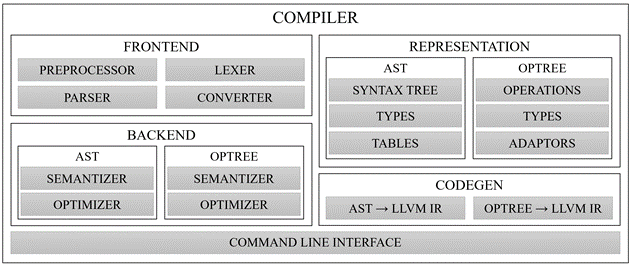
\includegraphics[width=\textwidth]{images/project-structure.png}
    \caption{Структура проекта.}
    \label{fig:project_structure}
\end{figure}

Для обеспечения корректности работы будет разработан комплект функциональных и интеграционных тестов для компонентов проекта.

Предполагается, что компилятор будет работать с Python-подобным статически типизированным языком, в котором будут присутствовать основные языковые конструкции (объявления функций и переменных, условия, циклы, вызовы функций, вычисление арифметико-логических выражений), возможность вывода текста на экран и считывания данных с клавиатуры.

В предлагаемой реализации компиляция кода должна осуществляться в несколько этапов.
За каждый из этапов отвечает один из представленных в рамках проекта модулей, взаимодействующих подобно конвейеру: выходные данные одного этапа являются входными для следующего, как это видно на рисунке~\ref{fig:compilation_pipeline}.
В предыдущей работе, упомянутой ранее, анализ компилируемой программы производился с использованием синтаксического дерева, что отражено в левой части схемы.
Теперь ему на смену пришло другое промежуточное представление – дерево операций, этапы анализа которого представлены справа.

\begin{figure}[h]
    \centering
    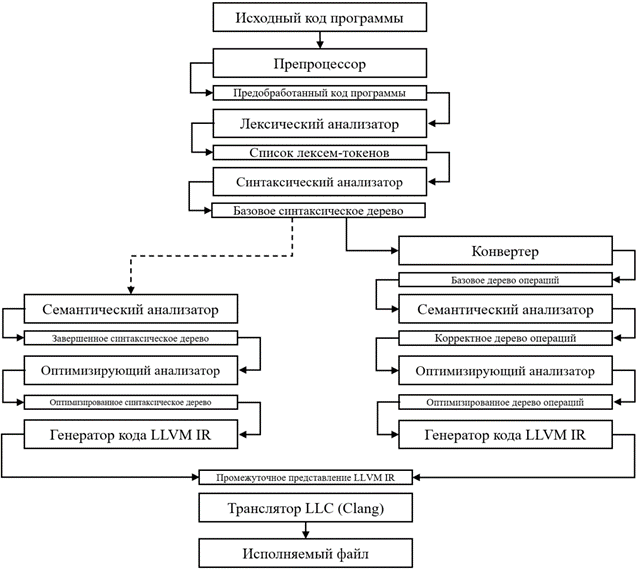
\includegraphics[width=\textwidth]{images/compilation-pipeline.png}
    \caption{Этапы компиляции.}
    \label{fig:compilation_pipeline}
\end{figure}

\newpage
\section{Компилируемый язык}
\label{sec:language}

Компилятор работает с простым языком программирования, основанным на Python 3 и Си.
Образно его можно охарактеризовать как «типизированный Python». Из Python был частично позаимствован синтаксис из-за его высокой читаемости и относительной простоты, а из Си - требования к объявлениям переменных и заголовкам функций.

\subsection{Идентификаторы}

Идентификаторами являются названия локальных переменных, названия функций, названия аргументов функций.
Правила именования состоят в следующем:

\begin{itemize}
    \item идентификатор обязан состоять из одного или более символов;
    \item идентификатор может состоять только из заглавных и строчных букв английского алфавита (A - Z, a - z), цифр от 0 до 9, знака нижнего подчеркивания \_;
    \item идентификатор не может иметь первым символом цифру от 0 до 9 (то есть, не может начинаться с цифры);
    \item идентификатор не может полностью совпадать с любым из ключевых слов языка.

\end{itemize}

Можно отметить, что в целом перечисленные правила справедливы для идентификаторов в языке программирования Си, поэтому с высокой вероятностью будут знакомы для пользователя компилятора.

\subsection{Ключевые слова}

Ключевые слова - это строго определенные последовательности символов - букв английского алфавита, которые служат для маркировки различных языковых конструкций, например, условных выражений.
Некоторые из ключевых слов также являются операторами, то есть, разделителями операндов в некоторых бинарных операциях.
Полный список зарезервированных слов, специальных для описываемого языка приведен в таблице ниже.

\begin{table}[h]
    \centering
    \caption{Ключевые слова}
    \label{tab:python_keywords}
    \begin{tabular}{>{\ttfamily}l p{11cm}}
        \toprule
        \textrm{\normalfont Ключевое слово} & \textrm{\normalfont Назначение}                                 \\
        \midrule
        and                                 & Оператор логической операции «и»                                \\
        bool                                & Название логического (булева) типа данных                       \\
        def                                 & Начало объявления функции                                       \\
        elif                                & Начало дополнительной ветки в ветвлении                         \\
        else                                & Начало альтернативной ветки в ветвлении                         \\
        False                               & Обозначение логического нуля или значения «ложь»                \\
        float                               & Название типа данных чисел с плавающей точкой                   \\
        for                                 & Начало циклической конструкции со счетчиком                     \\
        if                                  & Начало основной ветки в ветвлении                               \\
        int                                 & Название целочисленного типа данных                             \\
        None                                & Название типа данных, не содержащего значение                   \\
        or                                  & Оператор логической операции «или»                              \\
        return                              & Описание точки выхода из функции с возможным возвратом значения \\
        str                                 & Название строкового типа данных                                 \\
        True                                & Обозначение логической единицы или значения «истина»            \\
        while                               & Начало циклической конструкции с предусловием                   \\
        \bottomrule
    \end{tabular}
\end{table}

Кроме того, специфика языка подразумевает еще несколько зарезервированных слов, которые не являются «ключевыми» в полной мере, но интерпретация которых, тем не менее, не может контролироваться пользователем и также предопределена на уровне компилятора.
Такими словами являются:

\begin{itemize}
    \item \verb|main| - название функции - точки входа в программу. Любая программа на описываемом языке обязана иметь реализованную функцию main и ее выполнение начнется именно с этой функции.
    \item \verb|print| - название функции для вывода текста в стандартный поток вывода. Эта функция не может быть переопределена пользователем, и в месте ее упоминания в коде будет вставлен вызов функции printf из стандартной библиотеки языка Си.
    \item \verb|input| - название функции для получения текста из стандартного потока ввода. Эта функция также не может быть переопределена пользователем, и при трансляции будет использоваться функция scanf из стандартной библиотеки языка Си.
    \item \verb|range| - название выражения, напоминающего выхов функции и служащего для явного указания числа итераций в циклах со счетчиком.
    \item \verb|enumerate| - название выражения, напоминающего выхов функции и служащего для неявного указания числа итераций в циклах со счетчиком.
\end{itemize}

\subsection{Операторы}
\label{sec:operators}

Операторы - это определенные последовательности символов, как правило, короткие (состоящие из одного - двух знаков) и небуквенные, служащие преимущественно для отделения операндов в соответствующих операциях.
Многие из операций обозначаются привычными математическими символами и служат для написания арифметико-логических выражений, требуемых к вычислению в процессе выполнения программы.
Полный список значащих операторов и соответствующих им операций представлен в таблице ниже.

\begin{table}[h]
    \centering
    \caption{Операторы}
    \label{tab:operators}
    \begin{tabular}{>{\ttfamily}c p{12cm}}
        \toprule
        \textrm{\normalfont Оператор} & \textrm{\normalfont Назначение (операция)}   \\
        \midrule
        +                             & Сложение                                     \\
        -                             & Вычитание                                    \\
        *                             & Умножение                                    \\
        /                             & Деление или целочисленное деление            \\
        \%                            & Вычисление остатка от целочисленного деления \\
        =                             & Присваивание значения                        \\
        ==                            & Сравнение на равенство                       \\
        !=                            & Сравнение на неравенство                     \\
        >                             & Сравнение «больше»                           \\
        <                             & Сравнение «меньше»                           \\
        >=                            & Сравнение «больше или равно»                 \\
        <=                            & Сравнение «меньше или равно»                 \\
        \verb|[]|                     & Доступ к элементу списка                     \\
        \bottomrule
    \end{tabular}
\end{table}

Отдельно можно выделить круглые скобки: «(» и «)», служащие для группировки операндов в выражениях.
Кроме того, операторами являются ключевые слова «and» и «or», как уже было упомянуто ранее.
Операции имеют различный приоритет при вычислении, который, однако, преимущественно совпадает с общепринятым в математике.
Более подробно применение операторов будет рассмотрено в главе, посвященном синтаксическому анализу и разбору арифметико-логических выражений.

\subsection{Специальные последовательности}
\label{sec:special_sequences}

В языке также определено несколько специальных символьных последовательностей, которые трудно относить к операторам, хоть они и подходят под «внешнее» описание.
Тем не менее, специальные последовательности имеют особое назначение и однозначную интерпретацию.
Приведем их с описанием в таблице~\ref{tab:special_sequences}.

\begin{table}[h]
    \centering
    \caption{Специальные последовательности}
    \label{tab:special_sequences}
    \begin{tabular}{p{3cm}p{12cm}}
        \toprule
        \textbf{Написание}   & \textbf{Назначение}                                                                                                  \\
        \midrule
        \verb|,| (запятая)   & Разделитель аргументов в объявлениях функций, а также в их вызовах                                                   \\
        \addlinespace
        \verb|->| (стрелка)  & Разделитель между списком аргументов функции и типом возвращаемого значения                                          \\
        \addlinespace
        \verb|:| (двоеточие) & Разделитель имени и типа в объявлении переменных, а также выражения и тела (блока) в некоторых языковых конструкциях \\
        \bottomrule
    \end{tabular}
\end{table}

Дополнительно можно упомянуть последовательность из четырех пробелов, именуемую отступом и служащую для обозначения уровней вложенности в блоках кода.
Как и многие другие, эта последовательность была позаимствована из языка программирования Python, но в отличие от Python, число пробелов в ней должно быть фиксированным.

\subsection{Блоки кода}

Блоки в описываемом языке носят характер такой же, как и в других языках программирования, и служат для смыслового разделения частей программы по отношению к функциям и другим языковым конструкциям.
Выделение блоков кода аналогично тому, как это представлено в языке Python.
Каждая строка в программе может иметь в начале 0 или более отступов (см. п.~\ref{sec:special_sequences}).
Идущие непосредственно друг за другом строки считаются принадлежащими одному блоку тогда и только тогда, когда они имеют одинаковое количество отступов в начале.
Число отступов в начале каждой строки не может превышать число отступов в начале предыдущей строки более, чем на 1.
Таким образом, если в текущей строке число отступов на 1 больше, чем в предыдущей, то это значит, что она принадлежит новому блоку кода, вложенному в блок, которому принадлежит предыдущая строка.
Более наглядная демонстрация особенностей, связанных с блоками кода, будет представлена далее в примерах к описаниям языковых конструкций.

\subsection{Типы данных}
\label{sec:data_types}

Описываемый язык имеет определенную систему элементарных (базовых) типов для представления данных (преимущественно числовых) и работы с ними.
Как и в других языках программирования, каждый из типов характеризует множество допустимых значений данных, принадлежащих типу, и список операций, которые можно к ним применять.
Отдельно можно отметить, что представленная в языке типизация является статической, то есть, тип каждого значения, фигурирующего в коде и возникающего во время вычислений при исполнении программы, должен быть либо известен к началу компиляции, либо выведен к ее окончанию.
Все типы данных представлены в таблице~\ref{tab:data_types}.

\begin{table}[h]
    \centering
    \caption{Типы данных}
    \label{tab:data_types}
    \begin{tabular}{lp{3cm}p{7cm}p{3cm}}
        \toprule
        \textbf{Имя} & \textbf{Данные}                & \textbf{Значения}                                                                         & \textbf{Аналог в Си/C++}                     \\
        \midrule
        bool         & Логические значения            & True («истина») и False («ложь»)                                                          & bool                                         \\
        \addlinespace
        int          & Целые числа (8 байт)           & От $-9\,223\,372\,036\,854\,775\,808$ до $9\,223\,372\,036\,854\,775\,807$ (включительно) & \texttt{long int} или \texttt{std::int64\_t} \\
        \addlinespace
        float        & Числа с плавающей запятой      & От $\sim 1.7 \times 10^{-308}$ до $\sim 1.7 \times 10^{308}$                              & double                                       \\
        \addlinespace
        str          & Строки                         & Последовательность символов                                                               & \texttt{const char[] const}                  \\
        \addlinespace
        None         & Данные, не содержащие значения & Может принимать единственное значение None                                                & void                                         \\
        \bottomrule
    \end{tabular}
\end{table}

Как можно заметить, тип данных None не является типом в полной мере.
Он служит для обозначения типа возвращаемого значения у функций, которые не должны ничего возвращать.

Помимо элементарных типов, существует также составной тип, называемый list (список).
Он представляет собой последовательность значений, имеющих одинаковый элементарный тип (int или float).
Список имеет фиксированный размер, определяемый в момент его создания, но значения содержащихся в нем элементов могут изменяться в процессе исполнения программы.

\subsection{Арифметико-логические выражения}

Для декларирования необходимых при исполнении программы вычислений язык имеет полную поддержку арифметико-логических выражений, которые записываются в «обычной» (инфиксной) форме.
Выражения могут состоять из операторов, описанных в п.~\ref{sec:operators}, и операндов.
Операндами могут быть:

\begin{itemize}
    \item имена переменных, созданных (объявленных) по коду выше декларируемого выражения - в этом случае вместо имени переменной будет подставлено ее фактическое значение в момент вычисления выражения при выполнении программы;
    \item результаты вызовов функций - в этом случае будет скомпилирован вызов указанной в выражении подпрограммы с возможной передачей аргументов, и при исполнении программы в выражение попадет возвращенное значение;
    \item литеральные выражения или «литералы», то есть конкретные значения одного из встроенных в язык типов в символьной записи - в этом случае значение, которое необходимо подставить в выражение в качестве операнда при вычислении, считается известным на момент компиляции.
\end{itemize}

Для записи литеральных выражений каждого из типов определены некоторые правила.
Эти правила описаны в таблице~\ref{tab:literals}.

\begin{table}[h]
    \centering
    \caption{Литеральные выражения}
    \label{tab:literals}
    \begin{tabular}{lp{8cm}p{4cm}}
        \toprule
        \textbf{Тип данных} & \textbf{Описание записи}                                                                                                                                                     & \textbf{Примеры}  \\
        \midrule
        bool                & Два возможных значения, которые принадлежат этому типу, записываются, соответственно, как True («истина») и False («ложь»).                                                  & ---               \\
        \addlinespace
        int                 & Целые числа записываются с помощью набора символов - цифр от 0 до 9 без пробелов, перед которым дополнительно может находиться знак «минус» в случае отрицательных значений. & 1737, -56, 0      \\
        \addlinespace
        float               & Дробные значения с плавающей точкой записываются в виде десятичных дробей аналогично целым числам, для разделения целой и дробной части используется символ «точка».         & 1.3, -40.716, 0.0 \\
        \addlinespace
        str                 & Строки могут быть записаны в виде последовательности различных символов, обрамленных двойными кавычками.                                                                     & "A", "hello! W"   \\
        \addlinespace
        None                & Единственное значение, которое принадлежит типу, записывается как None.                                                                                                      & ---               \\
        \bottomrule
    \end{tabular}
\end{table}

Опишем также вставку вызова функции.
Вызов функции начинается с ее имени, далее следует пара круглых скобок, в которых через запятую перечисляются аргументы, которые необходимо передать в функцию.
Скобки обязательны, даже если функция не принимает аргументов.
Каждый из аргументов представляет собой отдельное арифметико-логическое выражение и, следовательно, так же может содержать в себе вызовы функций, другие допустимые операнды и операторы.

Внимания заслуживает также бинарная операция доступа к элементу списка.
Ее текстовое представление состоит из имени переменной и арифметико-логического выражения, указываемого далее в квадратных скобках, результатом которого должен являться номер (индекс) нужного элемента.
Нумерация элементов списка ведется с нуля.

\subsection{Объявление переменных}
\label{sec:var_declaration}

Переменные в языке программирования служат для хранения значений и могут быть использованы в арифметико-логических выражениях, в которые при этом будет подставлено фактическое значение переменной.
Отсюда следует, что каждая переменная характеризуется набором из трех компонентов, два из которых задаются при ее объявлении и не могут быть изменены в процессе выполнения программы:

\begin{itemize}
    \item имя (название) переменной (является идентификатором);
    \item тип данных, хранящихся в переменной;
    \item значение переменной (может меняться в процессе выполнения программы).
\end{itemize}

Переменные могут быть объявлены и при необходимости сразу определены (инициализированы) некоторыми значениями.
Инициализация переменных при объявлении не является обязательной, но рекомендуется во избежание возникновения неопределенного поведения при выполнении программы (к этому может привести, например, обращение к переменным, которые не были инициализированы при объявлении и которым не было присвоено какое-либо значение впоследствии).

Объявление переменной начинается с ее имени, далее следует разделитель (двоеточие) и имя типа (см. п.~\ref{sec:data_types}).
После этого может быть указано начальное значение переменной, предваряемое знаком равенства.
Каждое такое объявление должно начинаться на отдельной строке, при этом на одной строке не может быть более одного объявления переменной.
Следует также отметить, что имена переменных обязаны быть уникальными в пределах одного блока.
Нельзя переопределять переменные с одинаковыми названиями.

\begin{lstlisting}[language=Python, caption=Примеры объявлений переменных]
my_int: int = 5
another_int: int
my_float: float = 9.2
another_float: float = my_float * 4
\end{lstlisting}

Как видно из примеров, определение переменной может использовать значения ранее определенных переменных.
Переменные типа None явно объявлены быть не могут.

Отдельно стоит отметить объявление переменных-списков.
При указании типа такой переменной также указывается тип элементов списка в квадратных скобках.
В качестве инициализирующего значения, которое в случае списка обязано присутствовать в объявлении, может быть указана одна из следующих конструкций:

\begin{itemize}
    \item для списка с автоматическим выведением размера: значения элементов списка, разделенные запятыми и обрамленные квадратными скобками;
    \item для списка с размером, передаваемым с помощью арифметического выражения: значение, инициализирующее все элементы списка, в квадратных скобках, оператор умножения и выражение, определяющее размер списка.
\end{itemize}

\begin{lstlisting}[language=Python, caption=Примеры объявлений переменных типа list]
static_list: list[int] = [2, 4, 6, 8, 10]
dynamic_list: list[float] = [1.2] * 50
another_dynamic_list: list[int] = [0] * (a + b - 1)
\end{lstlisting}

\subsection{Объявление функций}

Подпрограммы, служащие для переиспользования кода по принципам процедурного программирования и повышения читаемости программы в целом, в описываемом языке представлены в виде функций.
Функции уже упоминались ранее при описании арифметико-логических выражений.
Объявление функции состоит из заголовка (сигнатуры) функции и ее реализации (определения).
Заголовок должен включать в себя:

\begin{itemize}
    \item имя (название) функции (является идентификатором);
    \item список аргументов (если они требуются);
    \item тип возвращаемого значения.
\end{itemize}

Список аргументов представляет собой, по сути, набор объявлений, схожих с объявлениями переменных, описанных в п.~\ref{sec:var_declaration}, перечисленных через запятую.
В каждом объявлении указывается имя переменной-аргумента, с которым она попадет в тело функции при ее вызове, и ее тип, разделенные двоеточием.

Таким образом, объявление функции начинается с ключевого слова def, затем следует имя. Далее идет список аргументов в паре круглых скобок.
Если функция не должна принимать аргументов, то указываются только открывающая и закрывающая круглые скобки.
После этого должна находиться специальная последовательность «стрелка» (см. п.~\ref{sec:special_sequences}) и название типа возвращаемого значения.
Если функция ничего не возвращает, следует указать тип None.
Заголовок функции заканчивается двоеточием, и с новой строки записывается тело (реализация) функции.
При этом оно должно находиться внутри отдельного (вложенного) блока кода, то есть, каждая строка обязана предваряться отступом.
Необходимо, чтобы тело функции содержало как минимум одну непустую строку.

\begin{lstlisting}[language=Python, caption=Примеры объявлений функций]
def func(arg1: int, arg2: float) -> float:
    x: int = arg1 + 3
    y: float = x - arg2
    return x * y

def another_func() -> int:
    return 3
\end{lstlisting}

Как можно заметить, передаваемые аргументы могут быть использованы непосредственно в выражениях без дополнительных объявлений в теле функции - достаточно их упоминания в заголовке.
Также, для указания возвращаемого значения используется ключевое слово return, за которым следует арифметико-логическое выражение.

\subsection{Условия (ветвления)}

Ветвление в программе может быть достигнуто при помощи особых языковых конструкций - условий.
Условие начинается с ключевого слова if, за которым следует проверяемое арифметико-логическое выражение и двоеточие.
После этого следует основная ветка - с новой строки в отдельном (вложенном) блоке указывается код, который должен быть выполнен, в случае если проверяемое условие окажется истинным в момент исполнения программы.
Если же условие будет ложным, то код основной ветки не будет выполнен и управление перейдет к командам после него.

При необходимости может быть добавлена альтернативная ветка - код в ней будет выполнен только в том случае, если проверяемое выражение окажется ложным.
Для этого используется ключевое слово else, за которым так же следует двоеточие.

Помимо этого, после основной ветки могут быть добавлены дополнительные, при чем у каждой из них будет «собственное» проверяемое выражение.
Такой «каскад» последовательно проверяемых веток записывается в коде практически так же, как и условие и тело основной ветки, с той лишь разницей, что для дополнительных веток используется ключевое слово elif вместо обычного if. Как следует из описания и специфики веток в конструкции условия (ветвления), части, начинающиеся с elif, должны идти после первой части, начинающейся с if, а часть, начинающаяся с else, может находиться только после них, то есть, в самом конце конструкции.

В каждом блоке в вышеперечисленных ветках, разумеется, могут находиться любые объявления переменных, арифметико-логические выражения, другие условные конструкции, а также циклы (см. п.~\ref{sec:loops}).
Таким образом, все языковые конструкции могут комбинироваться между собой в целях достижения требований к программе.

В примерах, приведенных далее, для простоты положим, что все используемые переменные объявлены и инициализированы некоторым корректным образом ранее в коде.

\begin{lstlisting}[language=Python, caption=Примеры условных конструкций]
if a == 1:
    b = 2

if c + 3 < d - 4:
    e: int = 5
    f = g - h
else:
    i = 6

if j >= 7 and k == 8.9:
    l = 10
elif m == 11:
    n: int = 12
elif o > 13.14 or p == 17:
    q: int = 5

if q > 0:
    q = 0
else:
    r = 15.16 + s
\end{lstlisting}

\subsection{Циклы}
\label{sec:loops}

В описываемом языке присутствует еще один род конструкций, присущих подходам структурного программирования -- это цикл.
Реализация поддерживает два вида циклов: цикл с предусловием и цикл со счетчиком. В общем случае цикл содержит преамбулу, определяющую проверяемое выражение, и непосредственно тело цикла -- код, который будет выполняться повторно до тех пор, пока вычисляемое перед каждым проходом цикла (итерации) выражение остается истинным.
В том случае, если выражение окажется ложным, цикл остановится и начнет выполняться код после описываемой конструкции.

Конструкция цикла с предусловием начинается с преамбулы: ключевого слова while, далее указывается контролируемое арифметико-логическое выражение, после этого идет двоеточие и, с новой строки, непосредственно тело цикла в отдельном (вложенном блоке).
Как и в случае с другими конструкциями, код в теле цикла может содержать в себе другие циклы, условия и прочие описанные ранее элементы языка.

В примерах, приведенных далее, для определенности будем считать, что все используемые переменные объявлены и инициализированы некоторым корректным образом ранее в коде.

\begin{lstlisting}[language=Python, caption=Пример цикла с предусловием]
while a != b or c < 17:
    a = a - 1
    c = c + d
\end{lstlisting}

Цикл со счетчиком устроен более сложно.
Преамбула начинается с ключевого слова for, далее указывается одна или две цикловые переменные, затем следуют: ключевое слово in, конструкция, регулирующая число итераций, и двоеточие.
С новой строки перечисляется тело цикла во вложенном блоке.
В описывемом языке поддерживаются три конфигурации цикла со счетчиком:

\begin{itemize}
    \item Явное указание числа итераций. Число итераций регулируется конструкцией вида \verb|range(|\(Start, Stop, Step\)\verb|)|, где все аргументы являются арифметико-логическими выражениями. Цикловой переменной является счетчик, изменяющийся в диапазоне от \(Start\) (включительно) до \(Stop\) (не включительно) с шагом \(Step\). Параметры \(Start\) и/или \(Step\) могут быть опущены, в этом случае они принимаются равными 0 и 1 соответственно.
    \item Обход списка по значениям. Число итераций регулируется конструкцией, состоящей из имени переменной-списка. В этом случае цикловой переменной является значение элемента из указанного списка, номер которого соответствует номеру итерации цикла.
    \item Обход списка по номерам (индексам) и значениям. Число итераций регулируется конструкцией вида \verb|range(|\(List\)\verb|)|, где \(List\) является именем переменной-списка. В этой конфигурации необходимо указывать две цикловые переменные, которым на каждой итерации будут присваиваться индекс и значение элемента списка соответственно.
\end{itemize}

\begin{lstlisting}[language=Python, caption=Примеры циклов со счетчиком]
for i in range(0, 10, 2):
    print(i)

for i in range(7):
    for j in range(1, a + b - 1):
        c = c + 1

for value in my_list:
    x = value - x

for i, value in enumerate(my_list):
    another_list[i] = value * 0.1
\end{lstlisting}

\subsection{Обобщение}

В заключение можно сделать вывод, что компилируемый язык представляет собой некоторую упрощенную вариацию существующих императивных языков программирования (Python, Си) и поддерживает многие конструкции, благодаря которым при написании программ на описываемом языке можно руководствоваться подходами процедурного (поддержка подпрограмм - функций) и структурного (наличие основных конструкций для линейного исполнения кода, ветвлений и циклов) программирования.
Тем не менее, в отличие от оригинального языка Python, в описанном языке отсутствует поддержка таких основных возможностей, как:

\begin{itemize}
    \item более сложные составные типы (словари, кортежи, списки с элементами различающихся типов);
    \item пользовательские типы (классы) и методы;
    \item обработка исключений;
    \item модули и импортирование библиотек.
\end{itemize}

\newpage
\section{Дерево операций}
\label{sec:optree}

\subsection{Актуальность применения подхода SSA}
\label{sec:optree_ssa}

Как уже было упомянуто, один из этапов компиляции -- синтаксический анализ.
Реализующий модуль, получая на вход список токенов, в качестве выхода строит синтаксическое дерево.
Такое дерево, помимо прочего, обладает определенными особенностями, среди которых были выделены преимущества и недостатки.

Преимущества:

\begin{itemize}
    \item Синтаксическое дерево легко строится напрямую из списка токенов (или даже текста программы, если лексический анализ совместить с построением дерева) за один проход фактически без дополнительных структур данных.
    \item Синтаксическое дерево является представлением входной программы один-в-один (текст программы может быть восстановлен путем полного обхода дерева), поэтому удобно предоставлять диагностику пользователю (указание точного места в исходном коде).
\end{itemize}

Недостатки:

\begin{itemize}
    \item Процесс семантического анализа дерева нетривиален. Требуется задействовать дополнительные структуры данных для упорядочения информации (список переменных, функций) и т. д.
    \item Применение существенных трансформаций (оптимизаций) является трудоемким: для обнаружения и проверки инвариантов требуется выполнять обходы по несколько раз (анализ использования переменных, вывод типов, поиск определений), что верно и для замены узлов дерева.
\end{itemize}

Для разрешения описанных трудностей, связанных, в частности, с анализом потока данных для выполнения трансформаций, было предложено использовать подход, похожий на SSA.

SSA (static single assignment, статическое единственное присвоение) -- это представление программы, в котором у каждой переменной есть единственное определение, сопровождающееся инициализацией.
Следующие примеры псевдокода демонстрируют одну и ту же программу, записанную в произвольной форме и в форме SSA.

\begin{lstlisting}[language=Python, caption=Программа в произвольной форме]
x = 1
y = x + 1
x = 2
z = x + 1
\end{lstlisting}

\begin{lstlisting}[language=Python, caption=Программа в форме SSA]
x1 = 1
y = x1 + 1
x2 = 2
z = x2 + 1
\end{lstlisting}

Используя свойство единственности присваивания, можно отследить, как было получено то или иное значение, обойдя цепочку определений и использований переменных.

В классическом подходе SSA, используемом в современных компиляторах, все высокоуровневые конструкции языка, такие как ветвления и циклы, разбиваются на последовательность базовых блоков программы, между которыми явно указываются переходы.
Кроме того, вводится понятие \(\phi\)-узлов, связывающих пути, по которым приходит определение переменной из разных блоков при нелинейном исполнении.
\cite{vladimirov}

В настоящей работе была реализована структура данных, использующая подход SSA в упрощенной форме, достаточной для достижения поставленных целей.
Эта структура, названная деревом операций, описана далее.

\subsection{Описание дерева операций}

Дерево операций -- это дополнительное промежуточное представление исходной программы.
В общем случае узлами дерева являются операции, которые обмениваются между собой значениями, каждое из которых определяется своим типом.
\cite{mlir_intro}

Как видно на рисунке~\ref{fig:optree_scheme}, операция может иметь произвольное число операндов, не более одного результата, произвольное число атрибутов (вспомогательных данных, независимых от других операций), произвольное число вложенных операций внутри, а также объемлющую операцию, в теле которой указанная операция и находится.

\begin{figure}[h]
    \centering
    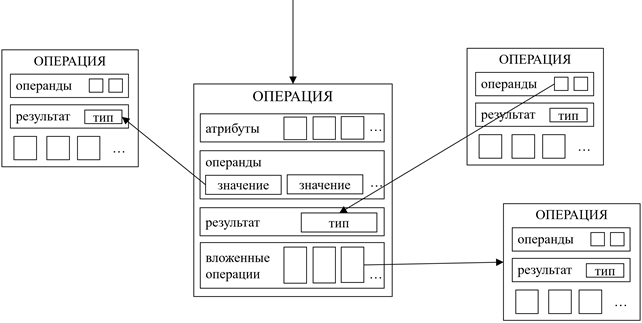
\includegraphics[width=\textwidth]{images/optree-scheme.png}
    \caption{Дерево операций.}
    \label{fig:optree_scheme}
\end{figure}

\textbf{Операция} владеет внешними значениями (результатами) и внутренними регистрами.
Результаты видны соседям операции и могут быть операндами других операций, но не видны операциям внутри тела.
Внутренние регистры, наоборот, доступны для использования операциями внутри тела, но снаружи не видны (как переменные во вложенном блоке в C++).
Операция не владеет операндами, так как это результаты или внутренние регистры других операций.
Также внутри хранится имя операции и код, определяющий ее вид (см. п.~\ref{sec:optree_rtti}).
Виды поддерживаемых операций представлены в п.~\ref{sec:optree_operations}.

\textbf{Значение} -- это единоразово определяемый неизменяемый регистр (как const переменная в C++).
Значение нельзя <<изменить>>, но можно создать новую операцию, которая будет иметь нужное значение в качестве результата, а старое значение отбросить (при необходимости удалить порождающую его операцию из дерева).
Значение хранит внутри себя породившую операцию, тип, список использований (операций, среди операндов которых есть указанное значение).

\textbf{Тип} -- это характеристика представления значения; неизменяемая структура, содержащая информацию, полезную для, собственно, представляемого типа.
Система типов в дереве операций сходна с системой типов компилируемого языка (см. п.~\ref{sec:optree_types}).

\textbf{Атрибут} -- это вспомогательные данные, которые используются для анализа операции (какое-либо численное значение, тип, подвид операции, строка и так далее).
Например, операция, описывающая функцию, может иметь имя функции и тип в качестве атрибутов, а операция, описывающая объявление константы - значение и тип константы и т. д.

К особенностям дерева операций можно отнести следующее:

\begin{itemize}
    \item Дерево операций можно построить из синтаксического дерева за один проход.
    \item Анализ использования значения представляет собой обход готового списка.
    \item Добавление или изменение операций прозрачно: операция хранит информацию о своем положении в дереве, значение хранит информацию о связанной операции и типе.
    \item Невозможно восстановить текст исходной программы напрямую, но можно ссылаться на исходный код в диагностике для пользователя, если сохранить ссылки на места в коде внутри операций при их создании из улов синтаксического дерева.
\end{itemize}

\subsection{Динамическая идентификация типов операций}
\label{sec:optree_rtti}

Динамическая идентификация типа данных (run-time type identification, RTTI) -- механизм в некоторых языках программирования, который позволяет определить тип данных переменной или объекта во время выполнения программы.
Существует множество реализаций такого механизма, но наиболее распространёнными являются:

\begin{itemize}
    \item таблица указателей на объекты;
    \item хранение информации об объекте в памяти вместе с ним.
\end{itemize}

Таким образом, операция определения типа сводится либо к поиску в таблице, либо к просмотру нескольких байт до адреса, на который указывает указатель на объект.
У каждого способа есть свои преимущества и недостатки.
К примеру, в первом случае для определения типа переменной требуется производить операции поиска по таблице указателей.
А во втором случае, переменные начинают занимать больше места в оперативной памяти, чем ожидается, ведь к их известному размеру добавляется некоторое количество байтов, нужных для идентификации их типа.

В настоящей работе для операций используется второй подход.
Для создания операций конкретного типа используются классы-адаптеры, каждый из которых представляет определенную операцию и имеет, помимо прочего, статический метод, возвращающий идентификатор типа операции.

\begin{lstlisting}[language=C++, caption=Фрагмент реализации RTTI]
struct ConcreteOp : public BaseOp {
    // ...

    static Operation::SpecId getSpecId() {
        static char specId = 0;
        return &specId;
    }

    static bool implementsSpecById(Operation::SpecId specId) {
        return specId == getSpecId() || BaseOp::implementsSpecById(specId);
    }
};
\end{lstlisting}

Таким образом, при создании конкретной операции в нее также записывается значение идентификатора типа операции из связанного адаптера.
Это позволяет реализовать для класса операции следующие методы, использующие RTTI:

\begin{lstlisting}[language=C++, caption=Интерфейс для доступа к RTTI]
struct Operation {
    using SpecId = void *;
    SpecId specId;
    // ...

public:
    template <typename AdaptorType> bool is() const;
    template <typename AdaptorType> AdaptorType as();
    template <typename AdaptorType> AdaptorType findParent() const;
    // ...
};
\end{lstlisting}

Эти методы позволяют проверить, является ли операция конкретной операцией, привести ее к указанному типу, а также найти в дереве операций среди предков узла операцию, имеющую определенный тип. Реализованный механизм применяется во многих компонентах проекта, работающих с деревом операций, например, в семантическом анализаторе.

\subsection{Система типов в дереве операций}
\label{sec:optree_types}

Для дерева операций была разработана система типов значений, схожая с системой типов данных компилируемого языка (см. п.~\ref{sec:data_types}).
Элементарные типы, наряду со связанными типами из компилируемого языка, представлены в таблице~\ref{tab:optree_basic_types}.

\begin{table}[h]
    \centering
    \caption{Элементарные типы}
    \label{tab:optree_basic_types}
    \begin{tabular}{lp{9cm}p{3cm}}
        \toprule
        \textbf{Название}  & \textbf{Описание}                      & \textbf{Связанный тип} \\
        \midrule
        \verb|IntegerType| & Целочисленное значение размером 8 байт & \verb|int|             \\
        \verb|BoolType|    & Целочисленное значение размером 1 байт & \verb|bool|            \\
        \verb|FloatType|   & Вещественное значение размером 8 байт  & \verb|float|           \\
        \verb|StrType|     & Массив символов размером по 1 байт     & \verb|str|             \\
        \verb|NoneType|    & Данные, не содержащие значения         & \verb|None|            \\
        \bottomrule
    \end{tabular}
\end{table}

Также присутствуют следующие составные типы:

\begin{itemize}
    \item \verb|FunctionType| -- функциональный тип.
          Используется для хранения заголовков функций, задается с помощью типа возвращаемого значения и списка типов аргументов.
    \item \verb|PointerType| -- внутреннее представление указателя.
          Используется для работы с переменными и списками, задается с помощью типа хранимого значения и, опционально, количества элементов, последовательно расположенных в памяти (размера списка).
\end{itemize}

\subsection{Обзор поддерживаемых операций}
\label{sec:optree_operations}

Каждая операция в дереве имеет название и идентификатор ее вида, определяющий ее назначение.
В общем случае, операция является абстракцией над одной или несколькими инструкциями в исполняемом файле, которые соответствуют ее семантике.
Например, арифметической бинарной операции обычно соответствует одна инструкция, вычисляющая результат заданной операции.
В то же время, операция, задающая цикл, при построении исполняемого файла должна быть развернута в целый набор вычислений и условных переходов.

Операции, реализованные в настоящей работе, можно разделить на несколько групп:

\begin{itemize}
    \item \textbf{Фундаментальные операции.}
          Операции в этой группе служат для задания основных "блоков" программы: объявления и вызова функций, введения констант.
          В группу входят следующие операции:
          \verb|ModuleOp, FunctionOp, FunctionCallOp, ReturnOp, ConstantOp|.
    \item \textbf{Вычислительные операции.}
          Эти операции являются репрезентацией вычисления всевозможных арифметико-логических выражений.
          В группу входят следующие операции:
          \verb|ArithBinaryOp, LogicBinaryOp, ArithCastOp, ArithUnaryOp, LogicUnaryOp|.
    \item \textbf{Операции по работе с памятью.}
          Указанной группе принадлежат операции, работающие с низкоуровневым представлением памяти для явной аллокации, загрузки и сохранения значений.
          В группу входят следующие операции:
          \verb|AllocateOp, LoadOp, StoreOp|.
    \item \textbf{Операции над потоком управления.}
          Операции в этой группе используются для декларирования условных и цикловых конструкций, а также их компонентов.
          В группу входят следующие операции:
          \verb|IfOp, ThenOp, ElseOp, WhileOp, ConditionOp, ForOp|.
    \item \textbf{Специальные операции.}
          Эти операции представляют собой высокоуровневые языковые конструкции, которые должны сохраниться и в низкоуровневом представлении.
          В группу входят следующие операции:
          \verb|InputOp, PrintOp|.
\end{itemize}

В соответствии со своим назначением, каждая операция обязана иметь заданное количество операндов, результирующих значений, внутренних регистров, атрибутов.
За проверку корректности этих, а также и других параметров, присущих операции, отвечает семантический анализатор, описанный в п.~\ref{sec:semantizer}.

\newpage
\section{Генератор промежуточного представления LLVM IR}
\label{sec:llvmir_codegen}

Для упрощения трансляции кода в машиночитаемый двоичный файл на этапе разработки компилятора можно частично «передать» эту задачу фреймворку LLVM.

\subsection{Актуальность использования LLVM}

LLVM (аббревиатура, может быть расшифрована как Low-Level Virtual Machine) - проект программной инфраструктуры для создания компиляторов и сопутствующих им утилит, который состоит из набора компиляторов языков высокого уровня (так называемых «фронтендов»), системы оптимизации, интерпретации и компиляции в машинный код.

Одна из особенностей фреймворка заключается в том, что он может создавать машинный код для множества архитектур, в том числе ARM, x86, x86-64, используя в качестве основы текст программы, написанный на языке промежуточного представления LLVM IR.
Этот язык представляет собой вариацию «высокоуровневого ассемблера», поддерживающего всевозможные арифметические и логические операции, работу с памятью, вызовы процедур, составные типы данных (структуры), манипуляции с регистрами и т. д.

Таким образом, для достижения поставленных в текущей практической работе задач можно выполнить все необходимые преобразования исходного кода на описанном в п.~\ref{sec:language} языке (предобработка, лексический анализ, синтаксический анализ, семантический анализ, итоговая оптимизация), затем путем обхода построенного дерева операций и выбора соответствующих инструкций LLVM IR создать текстовый файл, содержащий описанное промежуточное представление программы, и в итоге выполнить финальную трансляцию в объектный файл с помощью утилиты LLCompile (llc) из пакета LLVM.
Полученный файл может быть использован, например, компилятором clang или компоновщиком ld напрямую для связывания со стандартной библиотекой языка Си и получения исполняемого файла.

\subsection{Основной класс LLVMIRGenerator}

В программной реализации генератор промежуточного представления LLVM IR представлен в виде класса IRGenerator.
Содержательная часть объявления класса выглядит следующим образом:

\begin{lstlisting}[language=C++, caption=Объявление класса LLVMIRGenerator]
class LLVMIRGenerator {
  public:
    IRGenerator(const std::string &moduleName);
    void process(const SyntaxTree &tree);
    void writeToFile(const std::string &filename);
  private:
    llvm::Value *visitNode(Node::Ptr node);
    llvm::Value *visitBinaryOperation(Node *node);
    llvm::Value *visitFloatingPointLiteralValue(Node *node);
    llvm::Value *visitFunctionCall(Node *node);
    // ...
    void processNode(Node::Ptr node);
    void processExpression(Node *node);
    void processFunctionDefinition(Node *node);
    void processIfStatement(Node *node);
    // ...
};
\end{lstlisting}

Основным методом, выполняющим непосредственно генерацию кода, является process.
Этот метод принимает дерево операций, полученное в процессе компиляции (см. п.~\ref{sec:optree}).
Построенный код может быть в дальнейшем сохранен в файл с помощью метода writeToFile.

Принцип построения кода состоит в обходе синтаксического дерева и добавления инструкций с помощью соответствующего модуля из состава фреймворка LLVM.
Обход дерева производится рекурсивно от корня и начинается внутри метода process.
Как видно в представленном фрагменте кода, часть методов, отвечающих за обработку узлов дерева различных типов, имеют в названии префикс process или visit.
Особенность методов visit состоит в том, что они в результате просмотра узла возвращают вычислимое значение и используются для обхода арифметико-логических выражений.
Методы же, имеющие названия, начинающиеся со слова process, обходят узлы, которые по своей сути не являются частями выражений (например, конструкции с циклами и заголовки функций).

\subsection{Особенности реализации функций ввода-вывода}

В приведенном языке для ввода и вывода данных определены две «встроенные» функции print и input, реализация которых не может быть переопределена пользователем.
Тем не менее на самом деле обе они не имеют под собой реализации на этом языке, и в местах их вызова происходит обращение к стандартной библиотеке языка Си.

Более того, в силу специфики использования функции print и input можно считать в большей степени языковыми конструкциями, нежели функциями.
Функция print может принимать одно выражение любого из поддерживаемых типов в качестве аргумента (в языке C++, например, такое поведение функций называется перегрузкой), что для пользовательских функций запрещено.
Функция input ведет себя еще более нестандартно: она может находиться только в операциях присваивания и только в качестве правого операнда, при этом не принимает аргументов, но тип возвращаемого значения при ее вызове определяется типом переменной в роли левого операнда того же выражения (фигурально такое поведение можно назвать «перегрузкой по типу возвращаемого значения», по аналогии с обычными перегрузками из C++).

Рассмотрим теперь, каким образом вызовы этих функций компилируются во время генерации кода LLVM IR.

В месте вызова функции print происходит вставка инструкции LLVM IR, декларирующей вызов функции printf.
Как известно, эта функция принимает форматирующую строку и список выражений, тип которых должен совпадать с типами, соответствующим шаблонным последовательностям в форматирующей строке.
Таким образом, при генерации кода инструкция вызова printf содержит два передаваемых аргумента:

\begin{itemize}
  \item форматирующую строку, состоящую из одной шаблонной последовательности (типу int соответствует "\%d", типу float соответствует "\%lf", типу str соответствует "\%s", остальные типы содержат фиксированное множество значений и свою строку для каждого из значений: "True", "False", "None");
  \item значение выражения определенного типа, которое должно быть выведено в стандартный поток вывода (stdout).
\end{itemize}

В месте вызова функции input происходит аналогичная вставка вызова функции scanf.
Принцип использования этой функции отличается тем, что вместо значения выражения должен передаваться адрес переменной, в которую будет записано значение, полученное из стандартного потока ввода (stdin).

\newpage
\section*{Заключение}
\addcontentsline{toc}{section}{Заключение}

В результате выполнения выпускной квалификационной работы были достигнуты поставленные задачи, а именно:

\begin{itemize}
    \item определено подмножество реализуемого синтаксиса языка Python;
    \item изучена литература о структуре и способах разработки существующих компиляторов, а также моделях исполнения программ;
    \item разработана архитектура модулей компилятора и организация взаимодействия между ними для выбранного языка;
    \item реализован синтаксический анализатор и генератор промежуточного представления LLVM IR, произведено их тестирование.
\end{itemize}

Таким образом, был разработан и реализован компилятор.


% TODO: remove
\newpage
\section*{Тест библиографии}
\addcontentsline{toc}{section}{Тест библиографии}

dragonbook ~\cite{dragon_book}

llvmdocs ~\cite{llvm_docs}

mlirintro ~\cite{mlir_intro}

vladimirov ~\cite{vladimirov}


\newpage
\addcontentsline{toc}{section}{Список литературы}
\printbibliography

\end{document}
